\section{title}
	\section{Partial Differentiation and Gradients}
	\begin{tcolorbox}[colframe=defcolor,title={\color{white}\bf Partial Derivative}]
		\begin{definition}
			\[
			\fullfunction{f}{\R^n}{\R}{\vec{x}=(x_1,\cdots, x_n)}{y=f(\vec{x})}.
			\] \begin{align*}
			\pd{f}{x_1}&=\lim\limits_{h\to 0}\frac{f(x_1+h,x_2,\dots, x_n)-f(\vec{x})}{h}\\
			&\vdots\\
			\pd{f}{x_n}&=\lim\limits_{h\to 0}\frac{f(x_1,\dots,x_{n-1}, x_n+h)-f(\vec{x})}{h}\\
			\end{align*}
		\end{definition}
	\end{tcolorbox}
	\begin{remark}[Gradient]
		\[
		\nabla_{\vec{x}}f=\begin{bmatrix}
		\pd{f(\vec{x})}{x_1} & \pd{f(\vec{x})}{x_2} & \cdots & \pd{f(\vec{x})}{x_n}
		\end{bmatrix}\in M_{1\by n}(\R).
		\]
	\end{remark}
	
	\begin{example}

		\begin{align*}
		\od{g}{t}&=\pd{f}{x_1}\od{x_1}{t}+\pd{f}{x_2}\od{x_2}{t}\\
		&=\begin{bmatrix}
		\pd{f}{x_1} & \pd{f}{x_2}
		\end{bmatrix}\begin{bmatrix}
		\od{x_1}{t}\\ \od{x_2}{t}
		\end{bmatrix}\\
		&=\nabla f(x_1,x_2)\cdot\frac{\vec{x}}{dt}
		\end{align*}
		
		
		\begin{figure}[h!]\centering
			% https://tikzcd.yichuanshen.de/#N4Igdg9gJgpgziAXAbVABwnAlgFyxMJZARgBoAGAXVJADcBDAGwFcYkQAzEAX1PU1z5CKcqWLU6TVuwAeAfWI8+IDNjwEiAJjESGLNohDzNS-mqFEym3VIMgcPCTCgBzeEVAcAThAC2SUXsIJDIQAAsYeih2SDA2Xk8ff0RQnGDEAGYaCKiYgnjlbz8AmjSkbXDI6MNYgsTixAqyzOyqvLjHbiA
			\begin{tikzcd}
				& f \arrow[ld, no head] \arrow[rd, no head] &                         \\
				x_1 \arrow[rd, no head] &                                           & x_2 \arrow[ld, no head] \\
				& t                                         &                        
			\end{tikzcd}
		\end{figure}
	\end{example}
	
	
	\section{Gradients of Vector-Valued Functions}
	\[
	\fullfunction{\textbf{f}}{\R^n}{\R^m}{\vec{x}=\begin{bmatrix}
		x_1\\ \vdots\\ x_n
		\end{bmatrix}_{n\by 1}}{\vec{f}(\vec{x})=\begin{bmatrix}
		f_1(\vec{x})\\ \vdots\\ f_m(\vec{x})
		\end{bmatrix}=\begin{bmatrix}
		f_1(x_1,\cdots,x_n)\\ \vdots\\f_m(x_1,\cdots,x_n)
		\end{bmatrix}_{m\by 1}}
	\]
	\[
	\pd{\vec{f}}{x_i}=\lim\limits_{h\to0}\frac{\vec{f}(x_1,\cdots,x_i+h,\cdots,x_n)-\vec{f}()}{h}=\begin{bmatrix}
	\pd{f_1}{x_i} \\ \vdots\\ \pd{f_m}{x_i}
	\end{bmatrix}=
	\begin{bmatrix}
	\lim\limits_{h\to 0}\frac{f_1(x_1,\cdots,x_i+h,\cdots,x_n)-f_1(\vec{x})}{h}\\ \vdots\\ 
	\lim\limits_{h\to 0}\frac{f_m(x_1,\cdots,x_i+h,\cdots,x_n)-f_m(\vec{x})}{h}
	\end{bmatrix}\in\R^m
	\]
	\begin{tcolorbox}[colframe=defcolor,title={\color{white}\bf Jacobian}]
		\begin{definition}
			\begin{align*}
			\textbf{J}=\nabla_{\vec{x}}\vec{f}=\od{\vec{f}(\vec{x})}{\vec{x}}=
			\sbr{\pd{f_i}{x_i}}_{m\by n}&=\begin{bmatrix}
			\pd{\vec{f}\of{\vec{x}}}{x_1} &\cdots &
			\pd{\vec{f}\of{\vec{x}}}{x_n}
			\end{bmatrix}\\
			&=\begin{bmatrix}
			\pd{f_1(\vec{x})}{x_1} & \cdots & \pd{f_1(\vec{x})}{x_n}\\
			\vdots&\ddots&\vdots\\
			\pd{f_m(\vec{x})}{x_1} & \cdots & \pd{f_m(\vec{x})}{x_n}
			\end{bmatrix}
			\end{align*} \[
			\textbf{J}=\begin{cases}
			\begin{bmatrix}
			\pd{\vec{f}}{x_1} & \cdots & \pd{\vec{f}}{x_n}
			\end{bmatrix}\\
			\\
			\begin{bmatrix}
			\nabla f_1 & \cdots & \nabla f_m
			\end{bmatrix}^T
			\end{cases}
			\]
		\end{definition}
	\end{tcolorbox}
	\begin{remark}
		\ \begin{itemize}
			\item 
			The Jocobian approximates a nonlinear transformation locally with a linear transformation.
			\item The determinant of Jocobian $\approx$ scaling factor of Area/Volume
		\end{itemize}
	\end{remark}
	\newpage
	\begin{example}[\bf Gradient of a Least-Squares Loss in a Linear Model]
		Consider the linear model \[
		\vec{y}=\mvec{\Phi}\mvec{\theta},
		\] where \begin{enumerate}[(i)]
			\item $\mvec{\theta}\in\R^D$ is a parameter vector,
			\item $\mvec{\Phi}\in M_{N\by D}(\R)$ are input features and
			\item $\vec{y}\in\R^N$ are corresponding observations.
		\end{enumerate} Define the functions \begin{align*}
	L(\mvec{\varepsilon})&:=\mvec{\varepsilon}^T\mvec{\varepsilon}=\norms{\mvec{\varepsilon}}^2\\
	\mvec{\varepsilon}(\mvec{\theta})&:=\vec{y}-\mvec{\Phi}\mvec{\theta}.
\end{align*}
	\begin{figure}[h!]\centering
		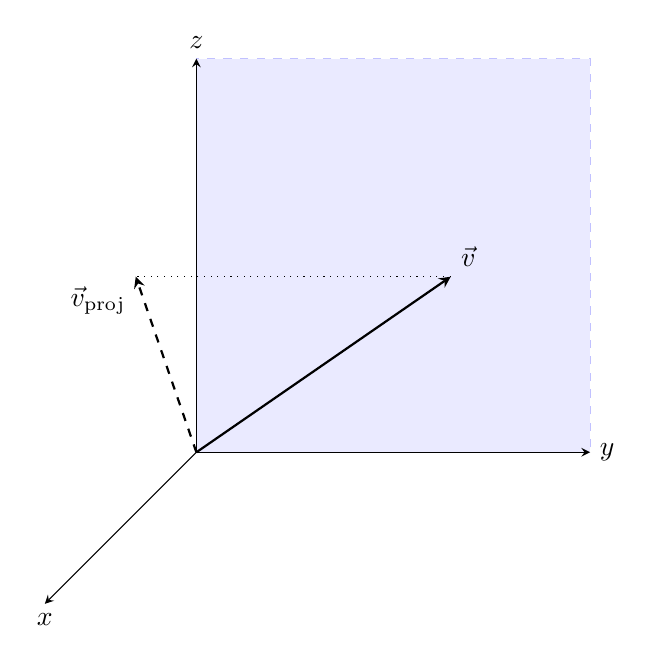
\begin{tikzpicture}[scale=1,transform shape,>=stealth]
		% Define main coordinates
		\coordinate (O) at (0,0,0);
		\coordinate (X) at (0,0,5);  % Previously Z
		\coordinate (Y) at (5,0,0);  % Previously X
		\coordinate (Z) at (0,5,0);  % Previously Y
		\coordinate (P) at (4,3,2);  % Vector in 3D
		\coordinate (P_proj) at (0,3,2);  % Its projection on the 2D plane (now the YZ plane)
		
		% Draw the plane (now the YZ plane)
		\filldraw[fill=blue!10,draw=blue!30,dashed,opacity=0.8] (O) -- (Y) -- (5,5,0) -- (Z) -- cycle;
		
		% Draw vector and its projection
		\draw[thick,->] (O) -- (P) node[above right] {$\vec{v}$};
		\draw[thick,->,dashed] (O) -- (P_proj) node[below left] {$\vec{v}_{\mathrm{proj}}$};
		\draw[dotted] (P) -- (P_proj);
		
		% Draw the axes
		\draw[->] (O) -- (X) node[below] {$x$};
		\draw[->] (O) -- (Y) node[right] {$y$};
		\draw[->] (O) -- (Z) node[above] {$z$};
		
		\end{tikzpicture}
	\end{figure}
	\end{example}
	
	\newpage
	\chapter{Probability and Distributions}
	
	\begin{tcolorbox}[colframe=defcolor,title={\color{white}\bf }]
		\begin{definition}
			
		\end{definition}
	\end{tcolorbox}
	\begin{tcolorbox}[colframe=thmcolor,title={\color{white}\bf }]
		\begin{theorem}
			
		\end{theorem}
	\end{tcolorbox}
